\chapter{Ugeopgave 9}
\label{cha:ugeopgave-9}

\section{Del 1}

Denne ugeopgave bruger samme \textit{framework} som ugeopgave 8.

\section{Del 2}

Vi reflekterer thepotten i vores plan der indeholder vores
``quad''. Vi skal spejle billedet ved at skifte orienteringen.

\section{Del 3}

Herefter blev der opsat endnu en lyskilde som bruges n�r vi tegner reflektionen.

\section{Del 4}

Vi sikrer os at \texttt{draw\_mirror} kaldes f�r
\texttt{draw\_proj\_shadow} i display
funktionen. \texttt{draw\_proj\_shadow} p�virker farve bufferen og denne
skal derfor sl�es fra og til f�r og efter funktionen
kaldes. \textit{Texturplanet} skal blendes med reflektionen af
tepotten. Resultatet kan ses i figur \ref{fig:9-1-1}.

\begin{figure}[hp]
\centering
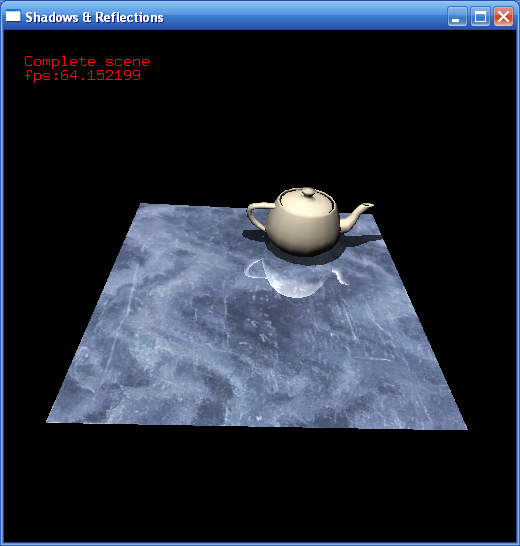
\includegraphics[width=8cm]{../exercise9/screenshots/4.png}
\caption{Tekande med reflektion}
\label{fig:9-1-1}
\end{figure}

\section{Del 5}

For at rette op p� den mindre fejl, at der kan blive tegnet reflektion
uden for reflektionsplanet, tegner vi f�rst reflektionsplanet. N�r
reflektionen s� skal tegnes bruger vi vores stencil buffer og tegner
derved kun reflektionen steder hvor der allerede er tegnet. Derved
undg�r vi at tegne uden for vores ``quad''


\section{Del 6}

Der st�r i opgaven at man skal lade tepotten g� igennem vores
``quad''. Det har den gjort siden del 1 i ugeopgave 8. Derved
opst�r der ikke noget nyt problem da vi allerede har taget h�jde for
dette med et clipping plane som vi introducerede i ugeopgave 8.

%%% Local Variables: 
%%% mode: latex
%%% TeX-master: "report_main"
%%% End: 